
\documentclass{beamer}

\usepackage{algpseudocode, color, colortbl, listings, MnSymbol}

\usepackage{hyperref}
\hypersetup{
    colorlinks=true,
    urlcolor=blue,
}

\usetheme{Montpellier}
\usecolortheme{rose}

% page numbers, from
% https://tex.stackexchange.com/questions/137022/how-to-insert-page-number-in-beamer-navigation-symbols
\expandafter\def\expandafter\insertshorttitle\expandafter{%
  \insertshorttitle\hfill%
  \insertframenumber\,/\,\inserttotalframenumber}

\definecolor{Gray}{gray}{0.8}
\newcolumntype{g}{>{\columncolor{Gray}}c}

\newcommand{\stanza}{ \\~\ }

\title{15. Approximate Set Cover and Bin Packing}
\subtitle{CPSC 535}
\author{Kevin A. Wortman}
\institute{ 
\includegraphics[height=2cm]{csuf-logo-cmyk} }
\date{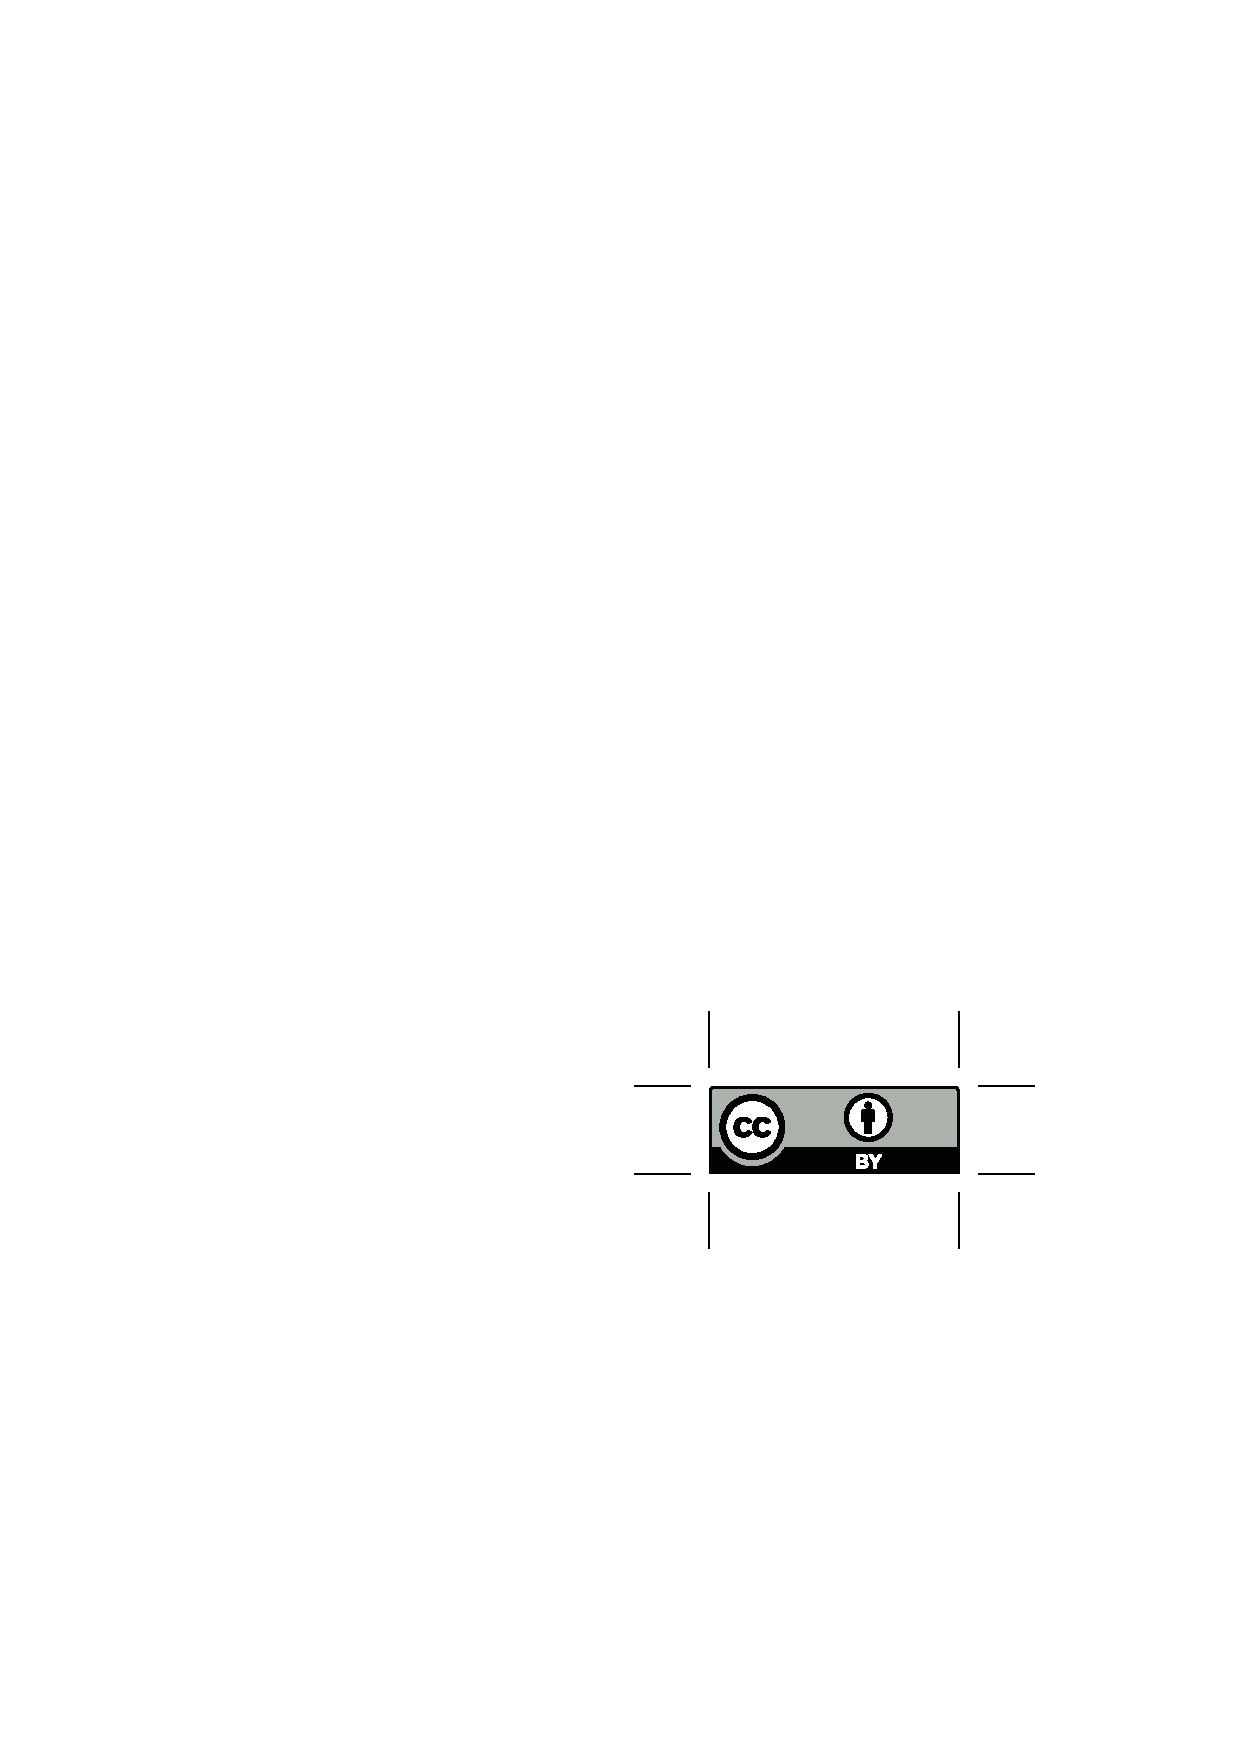
\includegraphics[height=14pt]{by} \\

{\tiny
This work is licensed under a
\href{http://creativecommons.org/licenses/by/4.0/}{Creative Commons Attribution 4.0 International License}.
}}

\begin{document}

\begin{frame}
  \titlepage
\end{frame}

\begin{frame} \frametitle{Set Cover: Intuition}
\begin{itemize}
  \item list of \textbf{needs}
  \item list of \textbf{services}
  \begin{itemize}
    \item each service meets some of the needs
  \end{itemize}
  \item \textbf{puzzle:} shortest list of products that meets all the needs?
\end{itemize}
\end{frame}

\begin{frame} \frametitle{Set Cover: Formal Definition}
  \emph{set cover problem} \\
  \textbf{input}: a universe set $X,$ and family $\mathfrak{F}$ of subsets of $X,$ such that $X=\bigcup_{S \in \mathfrak{F}} S$ \\
  \textbf{output}: a minimum size subfamily $\mathfrak{C} \subseteq \mathfrak{F}$ whose members cover all of $X,$ so
    $X = \bigcup_{S \in \mathfrak{C}} S$
\end{frame}

\begin{frame} \frametitle{Application: Streaming Services}
\begin{itemize}
  \item \textbf{needs:} stream TV shows $A, B, C, D, E, F$
  \item $X = \{A, B, C, D, E, F\}$
  \item \textbf{services:} alternative streaming services; each offer only some shows
  \item $\mathfrak{F} = \{ \{ A, F \}, \{A, C, E\}, \{B, E \}, \ldots \}$ 
  \item \textbf{puzzle:} subscribe to smallest number of services that provide all desired shows
\end{itemize}
\end{frame}

\begin{frame} \frametitle{Application: Menu Design}
  \begin{itemize}
    \item \textbf{needs:} menu has a food option available for various dietary needs
    \item $X = \{carnivore, vegan, kosher, halal, glutenfree, \ldots \}$
    \item \textbf{services:} alternative entrees
    \item $\mathfrak{F} = \{ \{ carnivore, halal \}, \{vegan\}, \{kosher, carnivore\}, \ldots \}$ 
    \item \textbf{puzzle:} design a menu with the fewest number of food options so that everyone can eat something
  \end{itemize}
\end{frame}
  
\begin{frame} \frametitle{Set Cover Hardness}
  \begin{itemize}
    \item set cover is $NP$-complete
    \item baseline algorithm: for each subset $\mathfrak{C} \subseteq \mathfrak{F},$ check if the sets in $\mathfrak{C}$ contain all elements, keep track of the smallest such $\mathfrak{C}$
    \item $\Theta(2^n \cdot n)$ time, slow
  \end{itemize}
\end{frame}

\begin{frame} \frametitle{Set Cover Approximation Algorithm}
  \begin{algorithmic}[1]
    \Function{APPROX-SET-COVER}{$X, \mathfrak{F}$}
      \State $U_0=\emptyset$ \Comment{still-uncovered elements}
      \State $\mathfrak{C} = \emptyset$
      \State $i=0$
      \While { $U_i \ne \emptyset$ }
        \State // choose set with most currently-uncovered elements
        \State Find $S \in \mathfrak{F}$ that maximizes $|S \cap U_i|$  
        \State $U_{i+1} = U_i - S$
        \State $\mathfrak{C} = \mathfrak{C} \cup \{S\}$
        \State $i = i + 1$
      \EndWhile
      \State \Return $\mathfrak{C}$
    \EndFunction
  \end{algorithmic}
\end{frame}

\begin{frame} \frametitle{Efficiency Analysis}
  \begin{itemize}
    \item while loop: $\Theta(n)$ iterations
    \begin{itemize}
      \item Find: $\Theta(n)$ time (assuming fast data structure to look up $U_i$)
      \item $U_{i+1} = U_i - S$: $\Theta(n)$ time
    \end{itemize}
    \item other steps: $\Theta(1)$ time each
    \item total time $\Theta(n^2)$ 
    \item can be sped up to $\Theta(n)$ (CLRS Exercise 35.3-3)
  \end{itemize}
\end{frame}

\begin{frame} \frametitle{Approximation Ratio}
\textbf{Theorem:} APPROX-SET-COVER is a $O(\lg n)$-approximation algorithm

Proof sketch:
\begin{itemize}
  \item Let $\mathfrak{C}^\star$ be the optimal cover and $k^\star=|\mathfrak{C}^\star|$
  \item $\mathfrak{C}^\star$ covers all of $X,$ and each $U_i \subseteq X$, so $\mathfrak{C}^\star$ covers each $U_i$
  \item each $U_i$ can be covered with $\leq k^\star$ sets from $\mathfrak{F}$
  \item on average, $\mathfrak{C}^\star$ covers $n/k^\star$ elements/set
  \item so at least one set in $\mathfrak{F}$ covers $\geq n/k^\star$ elements
  \item APPROX-SET-COVER picks the set that covers the most elements, so each $S$ covers at least $n/k^\star$ additional elements,
    and \[ U_{i+1} \leq |U_i| - |U_i|/k^\star = |U_i|(1-1/k^\star) \]
\end{itemize}
\end{frame}

\begin{frame} \frametitle{Approximation Ratio (continued)}
  \[ U_{i+1} \leq |U_i|(1-1/k^\star) \]
  \begin{itemize}
    \item algorithm stops when some $|U_i|=0$
    \item as a recurrence,
      \[ T(n) = (1-1/k^\star)n \]
    \item algebra and log rules show $T(n) \in O(k^\star \lg n)$
    \item each iteration adds one set to $\mathfrak{C}$, so APPROX-SET-COVER picks $O(k^\star \lg n)$ sets
    \item $k^\star$ is the optimal number of sets, so
    \item $\therefore$ APPROX-SET-COVER is a $O(\lg n)$-approximation algorithm $\qedsymbol$
  \end{itemize}
  \end{frame}
  
\begin{frame} \frametitle{Set Cover Summary}
\begin{itemize}
  \item set cover is $NP$-complete, exact algorithm takes exponential time
  \item fast $O(\lg n)$-approximate algorithm
  \item showed $\Theta(n^2)$ time
  \item $\Theta(n)$ time is possible
\end{itemize}
\end{frame}

\begin{frame} \frametitle{Big Idea: Linear Programming Relaxation}
Recall:
\begin{itemize}
  \item linear programming with real-valued variables is fast (polynomial time)
  \item integer linear programming (MIP) is $NP$-complete and slow (exponential time)
\end{itemize}

Idea:
\begin{itemize}
  \item formulate our problem as a MIP
  \item ``cheat'' and solve it as a LP
  \item round off each solution variable to the nearest integer
\end{itemize}
\end{frame}

\begin{frame} \frametitle{Big Idea: Linear Programming Relaxation}
\begin{itemize}
  \item \textbf{LP relaxation:} MIP formulation with integrality constraints removed
  \item not correct in general
  \item \textbf{but,} sometimes we can prove an approximate performance ratio
  \item next: algorithm that uses LP relaxation to solve vertex cover
\end{itemize}
\end{frame}

\begin{frame} \frametitle{Review: Vertex Cover}
  \emph{vertex cover problem} \\
  \textbf{input}: undirected graph $G=(V,E)$ \\
  \textbf{output}: set of vertices $C \subseteq V$, of minimal size $|C|,$ such
    that every edge in $E$ is incident on at least one vertex in $C$
   \stanza
  \begin{itemize}
    \item $NP$-complete
    \item previous deck: greedy algorithm, 2-approximate, $\Theta(m+n)$ time
  \end{itemize}
\end{frame}

\begin{frame} \frametitle{Vertex Cover Example}
  \begin{center}
    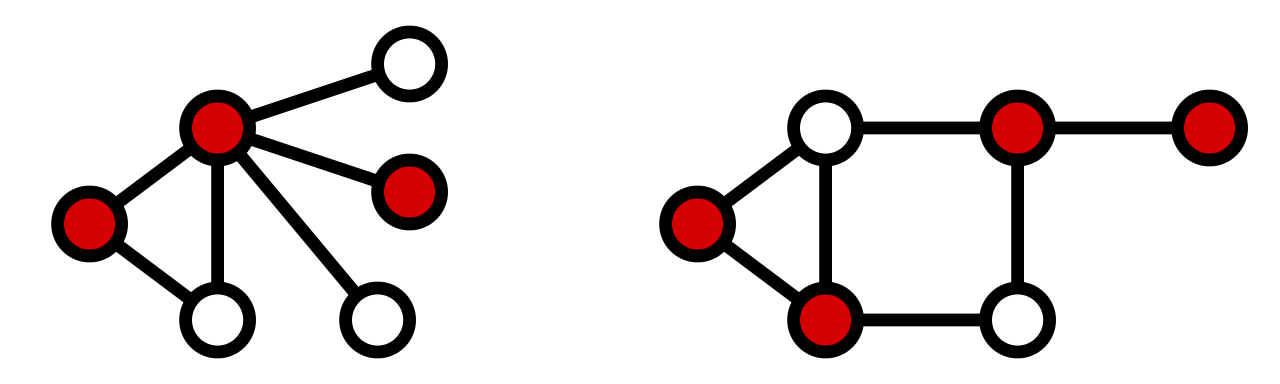
\includegraphics[height=80pt]{13-vertex-cover-1.png}
    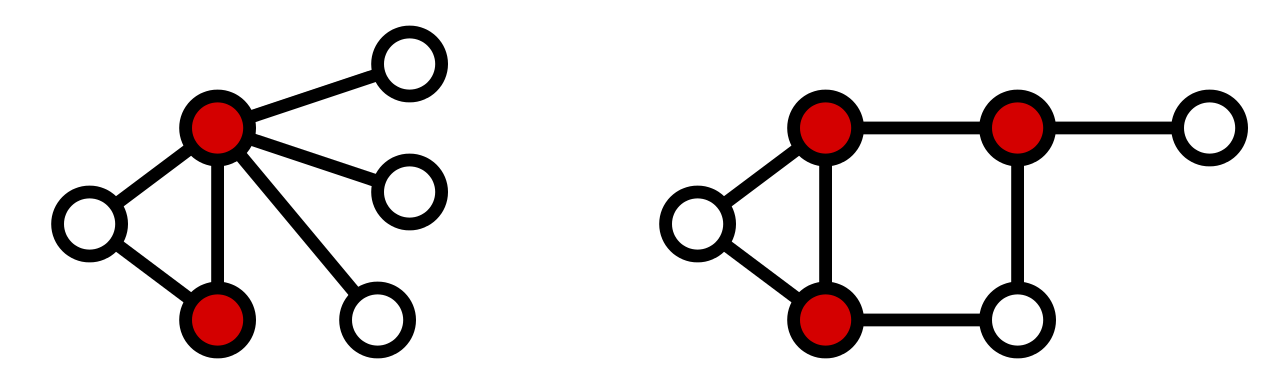
\includegraphics[height=80pt]{13-vertex-cover-2.png}
  \end{center}

  {\tiny
  Images credit: Wikipedia user Miym,
  \href{https://creativecommons.org/licenses/by-sa/3.0)}{CC BY-SA 3.0},
  \url{https://commons.wikimedia.org/wiki/File:Vertex-cover.svg},
  \url{https://commons.wikimedia.org/wiki/File:Minimum-vertex-cover.svg}
  }
\end{frame}

\begin{frame} \frametitle{Review: Formulating Vertex Cover}
  \textbf{Variables:} for each $v \in V$, create an integer variable $x_v$ such that
  \[ x_v = 1 \Leftrightarrow v \in C \]
  
  \textbf{Objective:} minimize
  \[ \sum_{v \in V} x_v \]
  
  \textbf{Constraints:}
  \begin{tabular}{lll}
    $0 \leq x_v \leq 1$ & $\forall v \in V$ & (0 or 1 indicator) \\
    $x_u + x_v \geq 1$ & $\forall (u, v) \in E$ & (each edge is covered)
  \end{tabular}
  
\end{frame}

\begin{frame} \frametitle{Review: Vertex Cover Outcomes}
  \begin{itemize}
    \item \textbf{Infeasible:}
      \begin{itemize}
      \item never happens
      \item $\exists$ a solution: setting all $x_v=1$ satisfies all constraints
      \end{itemize}
    \item \textbf{Unbounded:}
    \begin{itemize}
      \item never happens
      \item objective is bounded: the objective function is to minimize 
        \[ \sum_{v \in V} x_v; \]
        since every $x_v \geq 0$, the minimum objective value is zero, which is finite, so the program is never unbounded
    \end{itemize}
    \item \textbf{Solution:} Construct $C$ as
      \[ C = \{ v \,|\, v \in V \text{ and } x_v=1 \} \]
    \end{itemize}
\end{frame}

\begin{frame} \frametitle{Vertex Cover LP \underline{Relaxation}}
  \textbf{Variables:} for each $v \in V$, create a \underline{real-valued} variable $x_v$ such that
  \[ x_v = 1 \Leftrightarrow v \in C \]
  
  \textbf{Objective:} minimize
  \[ \sum_{v \in V} x_v \]
  
  \textbf{Constraints:}
  \begin{tabular}{lll}
    $0 \leq x_v \leq 1$ & $\forall v \in V$ & (\underline{fuzzy} 0 or 1 indicator) \\
    $x_u + x_v \geq 1$ & $\forall (u, v) \in E$ & (each edge is covered)
  \end{tabular}
  
\end{frame}

\begin{frame} \frametitle{LP Relaxation Vertex Cover Algorithm}
  \begin{algorithmic}[1]
    \Function{APX-VC-RELAX}{$G=(V,E)$}
      \State $C = \emptyset$
      \State $LP = $ the linear program from the previous slide
      \State $\bar{x} = SOLVE-LP(LP)$ \Comment{assume $LP$ has solution}
      \For{ each vertex $v \in V$ }
        \If{ $x_v \geq \frac{1}{2}$ } \Comment{ using $x_v \in \bar{x} $ }
          \State $C = C \cup \{v \}$
        \EndIf
      \EndFor
      \State \Return $C$
    \EndFunction
  \end{algorithmic}
\end{frame}

\begin{frame} \frametitle{Correctness}
\begin{itemize}
  \item $LP$ is never unbounded or infeasible
  \item must prove that $C$ is a valid vertex cover
  \item need, for each edge $\{u, v\} \in E,$ that $u \in C$ or $v \in C$ (or both)
  \item LP relaxation has constraints
    \begin{tabular}{lll}
      $x_u + x_v \geq 1$ & $\forall (u, v) \in E$ & (each edge is covered)
    \end{tabular}
  \item solution $\bar{x}$ satisfies all constraints, so
    \[  x_u + x_v \geq 1 \]
    is true and
    \[ x_u \geq \frac{1}{2} \text{ or } x_v \geq \frac{1}{2} \text{ (or both)}\]
  \item so the \textbf{for} loop adds at least one of $u, v$ to $C$
\end{itemize}
\end{frame}

\begin{frame} \frametitle{Efficiency Analysis}
  \begin{itemize}
    \item create $LP:$ $\Theta(n+m)$
    \item solve $LP:$ polynomial
    \item post-processing \textbf{for} loop: $\Theta(n)$
    \item total time
      \[ \Theta(n+m) + \Theta(\text{solve LP}) + \Theta(n) = \Theta(\text{solve LP}) \]
    \item polynomial time
  \end{itemize}
\end{frame}

\begin{frame} \frametitle{Approximation Ratio}
  \textbf{Theorem:} APX-VC-RELAX is a 2-approximation algorithm

  Proof sketch:
  \begin{itemize}
    \item let $C^\star$ be an optimal vertex cover for $G$
    \item need to prove $|C| \leq 2 |C^\star|$
    \item use a ``common ground'' comparison between $|C|$ and $|C^\star|$
    \item let
      \begin{align*}
        z^\star &= \text{objective function value of LP} \\
        &= \sum_{v \in V} x_v \text{ using each } x_v \in \bar{x}
      \end{align*}
    \item we use $z^\star$ to relate $|C|$ to $|C^\star|$
  \end{itemize}
\end{frame}

\begin{frame} \frametitle{Relating $z^\star$ to $|C^\star|$}
  \begin{itemize}
    \item $z^\star$ is objective value $f(C)$ for our relaxed LP
    \item $C^\star$ is solution to MIP, with more constraints (integer $x_v$)
    \item so
      \begin{align*}
        z^\star &\leq f(C^\star) \\
          &= |C^\star|
      \end{align*}
  \end{itemize}
\end{frame}

\begin{frame} \frametitle{Relating $z^\star$ to $|C|$}
  \begin{itemize}
    \item now relate $z^\star$ to $|C|:$
      \begin{align*}
        z^\star &= \sum_{v \in V} x_v \\
          &\geq \sum_{v \in V, x_v \geq 1/2} x_v \\
          &\geq \sum_{v \in V, x_v \geq 1/2} (\frac{1}{2}) \\
          &= \sum_{v \in C} \frac{1}{2} \\
          &= \frac{1}{2} |C|
      \end{align*}
\end{itemize}
\end{frame}

\begin{frame} \frametitle{Completing the Proof of Approximation Ratio}
  Combine
  \[ z^\star \leq |C^\star| \]
  with
  \[ z^\star \geq \frac{1}{2} |C| \]
  to obtain
  \[ \frac{1}{2} |C| \leq z^\star \leq |C^\star| \]
  or
  \[ |C| \leq 2 \cdot |C^\star| . \]

  QED.
\end{frame}

\begin{frame} \frametitle{Vertex Cover LP Relaxation Summary}
\begin{itemize}
  \item LP relaxation approach:
    \begin{itemize}
      \item formulate vertex cover as MIP
      \item remove integer constraints, solve as LP
      \item round each solution variable to nearest integer
    \end{itemize}
  \item same polynomial runtime as linear programming
  \item 2-approximation
  \item compared to greedy algorithm in previous slides, this algo. is
  \begin{itemize}
    \item simpler
    \item slower
  \end{itemize}
  \item generalizes to \textbf{weighted} case (see textbook section 35.5)
\end{itemize}
\end{frame}

\begin{frame} \frametitle{Bin Packing: Intuition}
  \begin{itemize}
    \item have a collection of \textbf{items}
    \item want to \textbf{pack} them tightly into containers
    \item \textbf{puzzle}: which items go together in each container?
  \end{itemize}
\end{frame}

\begin{frame} \frametitle{Bin Packing: Formal Definition}
  \emph{bin packing problem} \\
  \textbf{input}: a multiset $U = \{u \in \mathbb{Q}, 0 < u\leq 1\}$ of item sizes \\
  \textbf{output}: a partition $B_1, B_2, \ldots, B_k$ of $U$ into $k$ multisets, such that the sum of each $B_i$ is at most 1
  \stanza

  \begin{itemize}
    \item bin capacity is 1
    \item each size $u \in U$ is a fraction between 0 and 1
    \item ex. $U=\{\frac{2}{3}, \frac{1}{2}, \frac{1}{9}, \frac{1}{2}, \ldots \}$
    \item $k = \text{number of bins used}$
  \end{itemize}
\end{frame}

\begin{frame} \frametitle{Example Applications}
  \begin{itemize}
    \item Given a sink full of dirty dishes, how to load the dishwasher to clean all the dishes in the fewest loads?
    \item Given an Amazon order for items of varying weights, how to pack the items into the fewest shipping boxes?
    \item Given a set of virtual machines (VMs) of varying memory sizes, how to host them on the fewest physical servers?
  \end{itemize}
\end{frame}

\begin{frame} \frametitle{Generalizations of Bin Packing}
  Problem statement can be generalized to be more realistic:
  \begin{itemize}
    \item items are 2D shapes instead of numbers (physical object shipping)
    \item items can partially overlap (VM shared memory can overlap)
    \item one bin, different values: \emph{knapsack problem}
    \item minimize bins, and also waste: \emph{cutting stock problem}
  \end{itemize}
\end{frame}

\begin{frame} \frametitle{Bin Packing Hardness}
  \begin{itemize}
    \item bin packing is $NP$-complete
    \item generalizations (ex. 2D shapes) are even harder
    \item baseline algorithm:
      \begin{itemize}
        \item loop through each possible number of bins $k=1, \ldots, n$
        \item for each item $u \in U:$ try placing $u$ in all $k$ bins, then recursively place the remaining items
      \end{itemize}
    \item $\Theta(n \cdot n!)$ time, extremely slow
    \item (exponential time is possible too)
  \end{itemize}
\end{frame}

\begin{frame} \frametitle{Greedy Algorithm Idea}
  \begin{itemize}
    \item keep a list of bins
    \item for each item $u:$ find any bin with enough room for $u,$ and put it there
    \item if no bin has enough room: start a new bin holding just $u$
    \item \textbf{``first fit''} algorithm
  \end{itemize}
\end{frame}

\begin{frame} \frametitle{First-Fit Algorithm}
  {\footnotesize
  \begin{algorithmic}[1]
    \Function{FIRST-FIT-BIN-PACK}{$U$}
      \State $B = \emptyset$ \Comment{the bins}
      \For{ $u \in U$ }
        \State $packed = false$
        \For{ $B_i \in B$ }
          \If{ $(u + \sum B_i ) \leq 1$ } \Comment{ does $u$ fit in $B_i$? }
            \State $B_i = B_i \cup \{ u \}$
            \State $packed = true$
            \State \textbf{break} loop
          \EndIf
        \EndFor
        \If{ $packed == false$ }
          \State $B_k = \{ u \} $ \Comment{$u$ in its own new bin}
          \State $B = B \cup \{ B_k \}$
        \EndIf
      \EndFor
      \State \Return $B$
    \EndFunction
  \end{algorithmic}
  }
\end{frame}

\begin{frame} \frametitle{Efficiency Analysis}
\begin{itemize}
  \item outer \textbf{for} loop: $\Theta(n)$ iterations
  \item $|B| \leq n$, so
  \item inner \textbf{for} loop: $\Theta(n)$ iterations
  \item $\sum B_i: \Theta(n)$ time
  \item other statements are $\Theta(1)$ time
  \item $\therefore \enspace \Theta(n^3)$ total time
  \item can speed up to $\Theta(n \log n)$ by caching totals and storing bins in a BST
\end{itemize}
\end{frame}

\begin{frame} \frametitle{Approximation Ratio}
\textbf{Theorem}: FIRST-FIT-BIN-PACK is a 2-approximation algorithm.

Proof sketch:
\begin{itemize}
  \item Recall $k=|B|$
  \item Let $B^\star$ be an optimal multiset of bins, and $k^\star=|B^\star|$
  \item (again) use ``common ground'' comparison between $k$ and $k^\star$
  \item Let $t = \sum U$ be the sum of all items; use $t$ as common ground
  \item Best possible packing fills every single bin with no leftover space, so
    \[ k^\star \geq \frac{\text{total size of items}}{\text{size of each bin}} = \frac{(t)}{(1)} = t \]
\end{itemize}
\end{frame}

\begin{frame} \frametitle{There Is At Most One Light Bin}
  \begin{itemize}
    \item Call a bin $B_i$ \textbf{``light''} when $\sum B_i \leq \frac{1}{2},$ otherwise \textbf{``heavy''}
    \item Invariant: there is at most one light bin
    \item Induction on number of items in bins
    \item Base case: zero items $\implies$ zero bins $\implies$ no light bin
    \item Inductive case: given new item $u,$ four cases:
  \end{itemize}
  \begin{center}
  \begin{tabular}{l | p{1in} | p{1in} }
        & $u \leq \frac{1}{2}$ & $u > \frac{1}{2}$ \\ \hline
        no light bin & $u$ starts only light bin & $u$ starts new heavy bin \\ \hline
        $\exists$ light bin $B_i$ & $u$ joins $B_i$ & $u$ either joins $B_i$ making it heavy; or starts a new heavy bin \\ \hline
  \end{tabular}
  \end{center}
  \end{frame}
    
\begin{frame} \frametitle{Approximation Ratio (continued)}
  \begin{itemize}
    \item worst case is one light bin and $k-1$ barely-heavy bins
    \item $k$ is at most
      \[ k \leq \frac{\text{total size of items}}{\text{size of each bin}} + 1 < \frac{(t)}{(1/2)} + 1 = 2t+1 \]
    \item we showed $k^\star \geq t,$ so
      \[ k < 2t+1 \leq 2(k^\star)+1 \]
    \item for large $n,$
      \[ k \propto 2 k^\star \]
    \item QED
  \end{itemize}
\end{frame}
    
\begin{frame} \frametitle{Tight Approximation Ratio}
  \begin{itemize}
    \item (Johnson, Demers, Ullman, Garey, Graham 1974)
    \item FIRST-FIT-BIN-PACK is a 1.7-approximation algorithm
    \begin{itemize}
      \item More elaborate case analysis
    \end{itemize}
    \item There is a $U$ for which FIRST-FIT-BIN-PACK achieves only a 1.7 performance ratio
    \begin{itemize}
      \item $U = \{ \frac{6}{101} \times 7, \frac{10}{101} \times 7, \frac{16}{101} \times 3, \frac{34}{101} \times 10, \frac{51}{101} \times 10 \}$
      \item $k^\star = 10$
      \item $k = 17$
    \end{itemize}
    \item $\therefore \enspace$ the $1.7 k^\star$ bound is tight
  \end{itemize}
\end{frame}

\begin{frame} \frametitle{Bin Packing Summary}
\begin{itemize}
  \item bin packing is $NP$-complete, exact algorithm takes exponential time
  \item $\Theta(n \log n)$ time, 1.7-approximation algorithm
  \item we only proved $\Theta(n^3)$ time, 2-approximation
\end{itemize}
\end{frame}


\end{document}
